\Exhibit{BeamGitHubStars}{%
    Screenshot of the top 1.2\% repositories of \Asf featuring Beam%
}

This is a screenshot of the GitHub page with all code repositories owned by \Asf.
It is sorted by the number of starts, from highest to lowest.

The `beam' repository of Apache Beam is seen at the bottom of the first page of 85 pages in total.
According to this screenshot, this repository is 30th by the number of stars.

GitHub stars is a valid metric of software popularity as explained in \ExhibitRef{GitHubStars}.

The address on this screenshot already forces sorting by the number of stars,
but you can additionally verify the sorting by selecting `Sort' \textbackslash `Stars'
in the dropdown near the top of the page.

Note: By the time you will be verifying this screen, the `beam' repository may slide down to the second page.
If you cannot find it at the bottom of the first page, please check the second page as well.

\begin{center}
    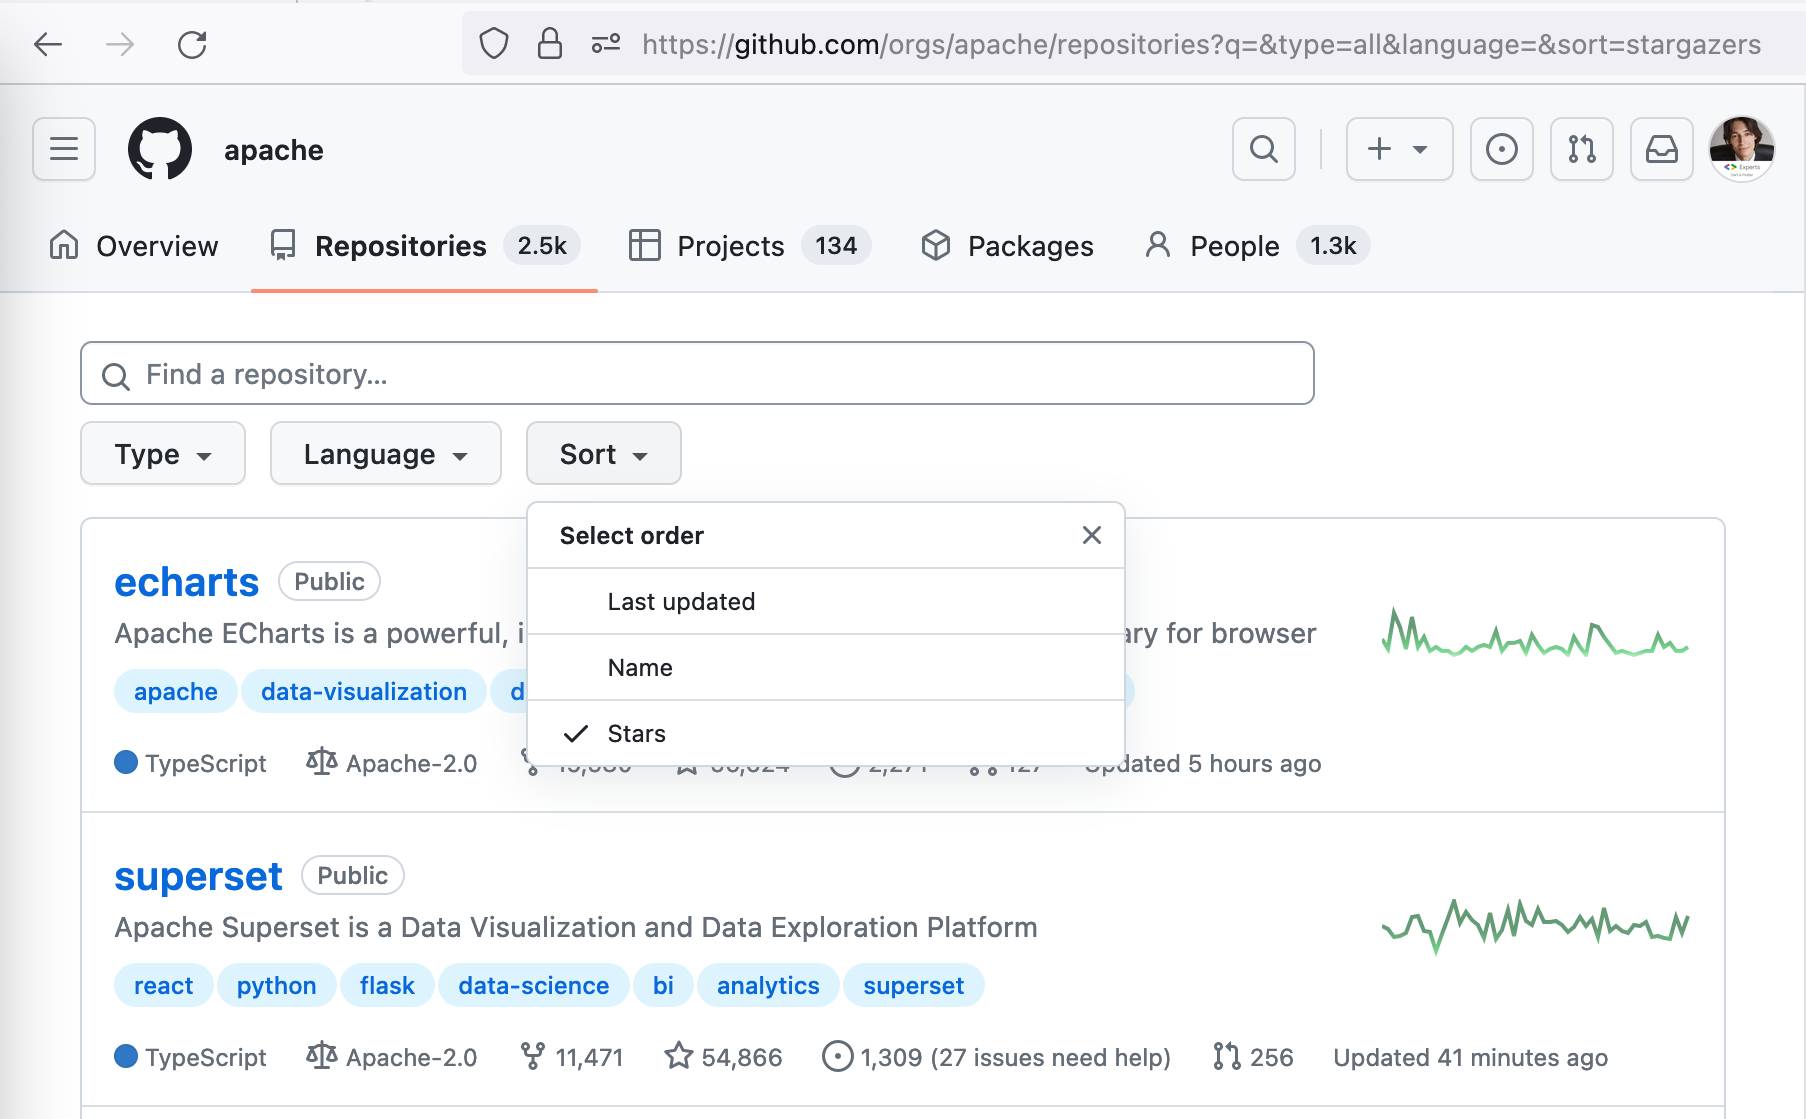
\includegraphics[width=40em]{beam-github-stars-dropdown-p1}
\end{center}
\WillContinue
\pagebreak

\Continuing
\begin{center}
    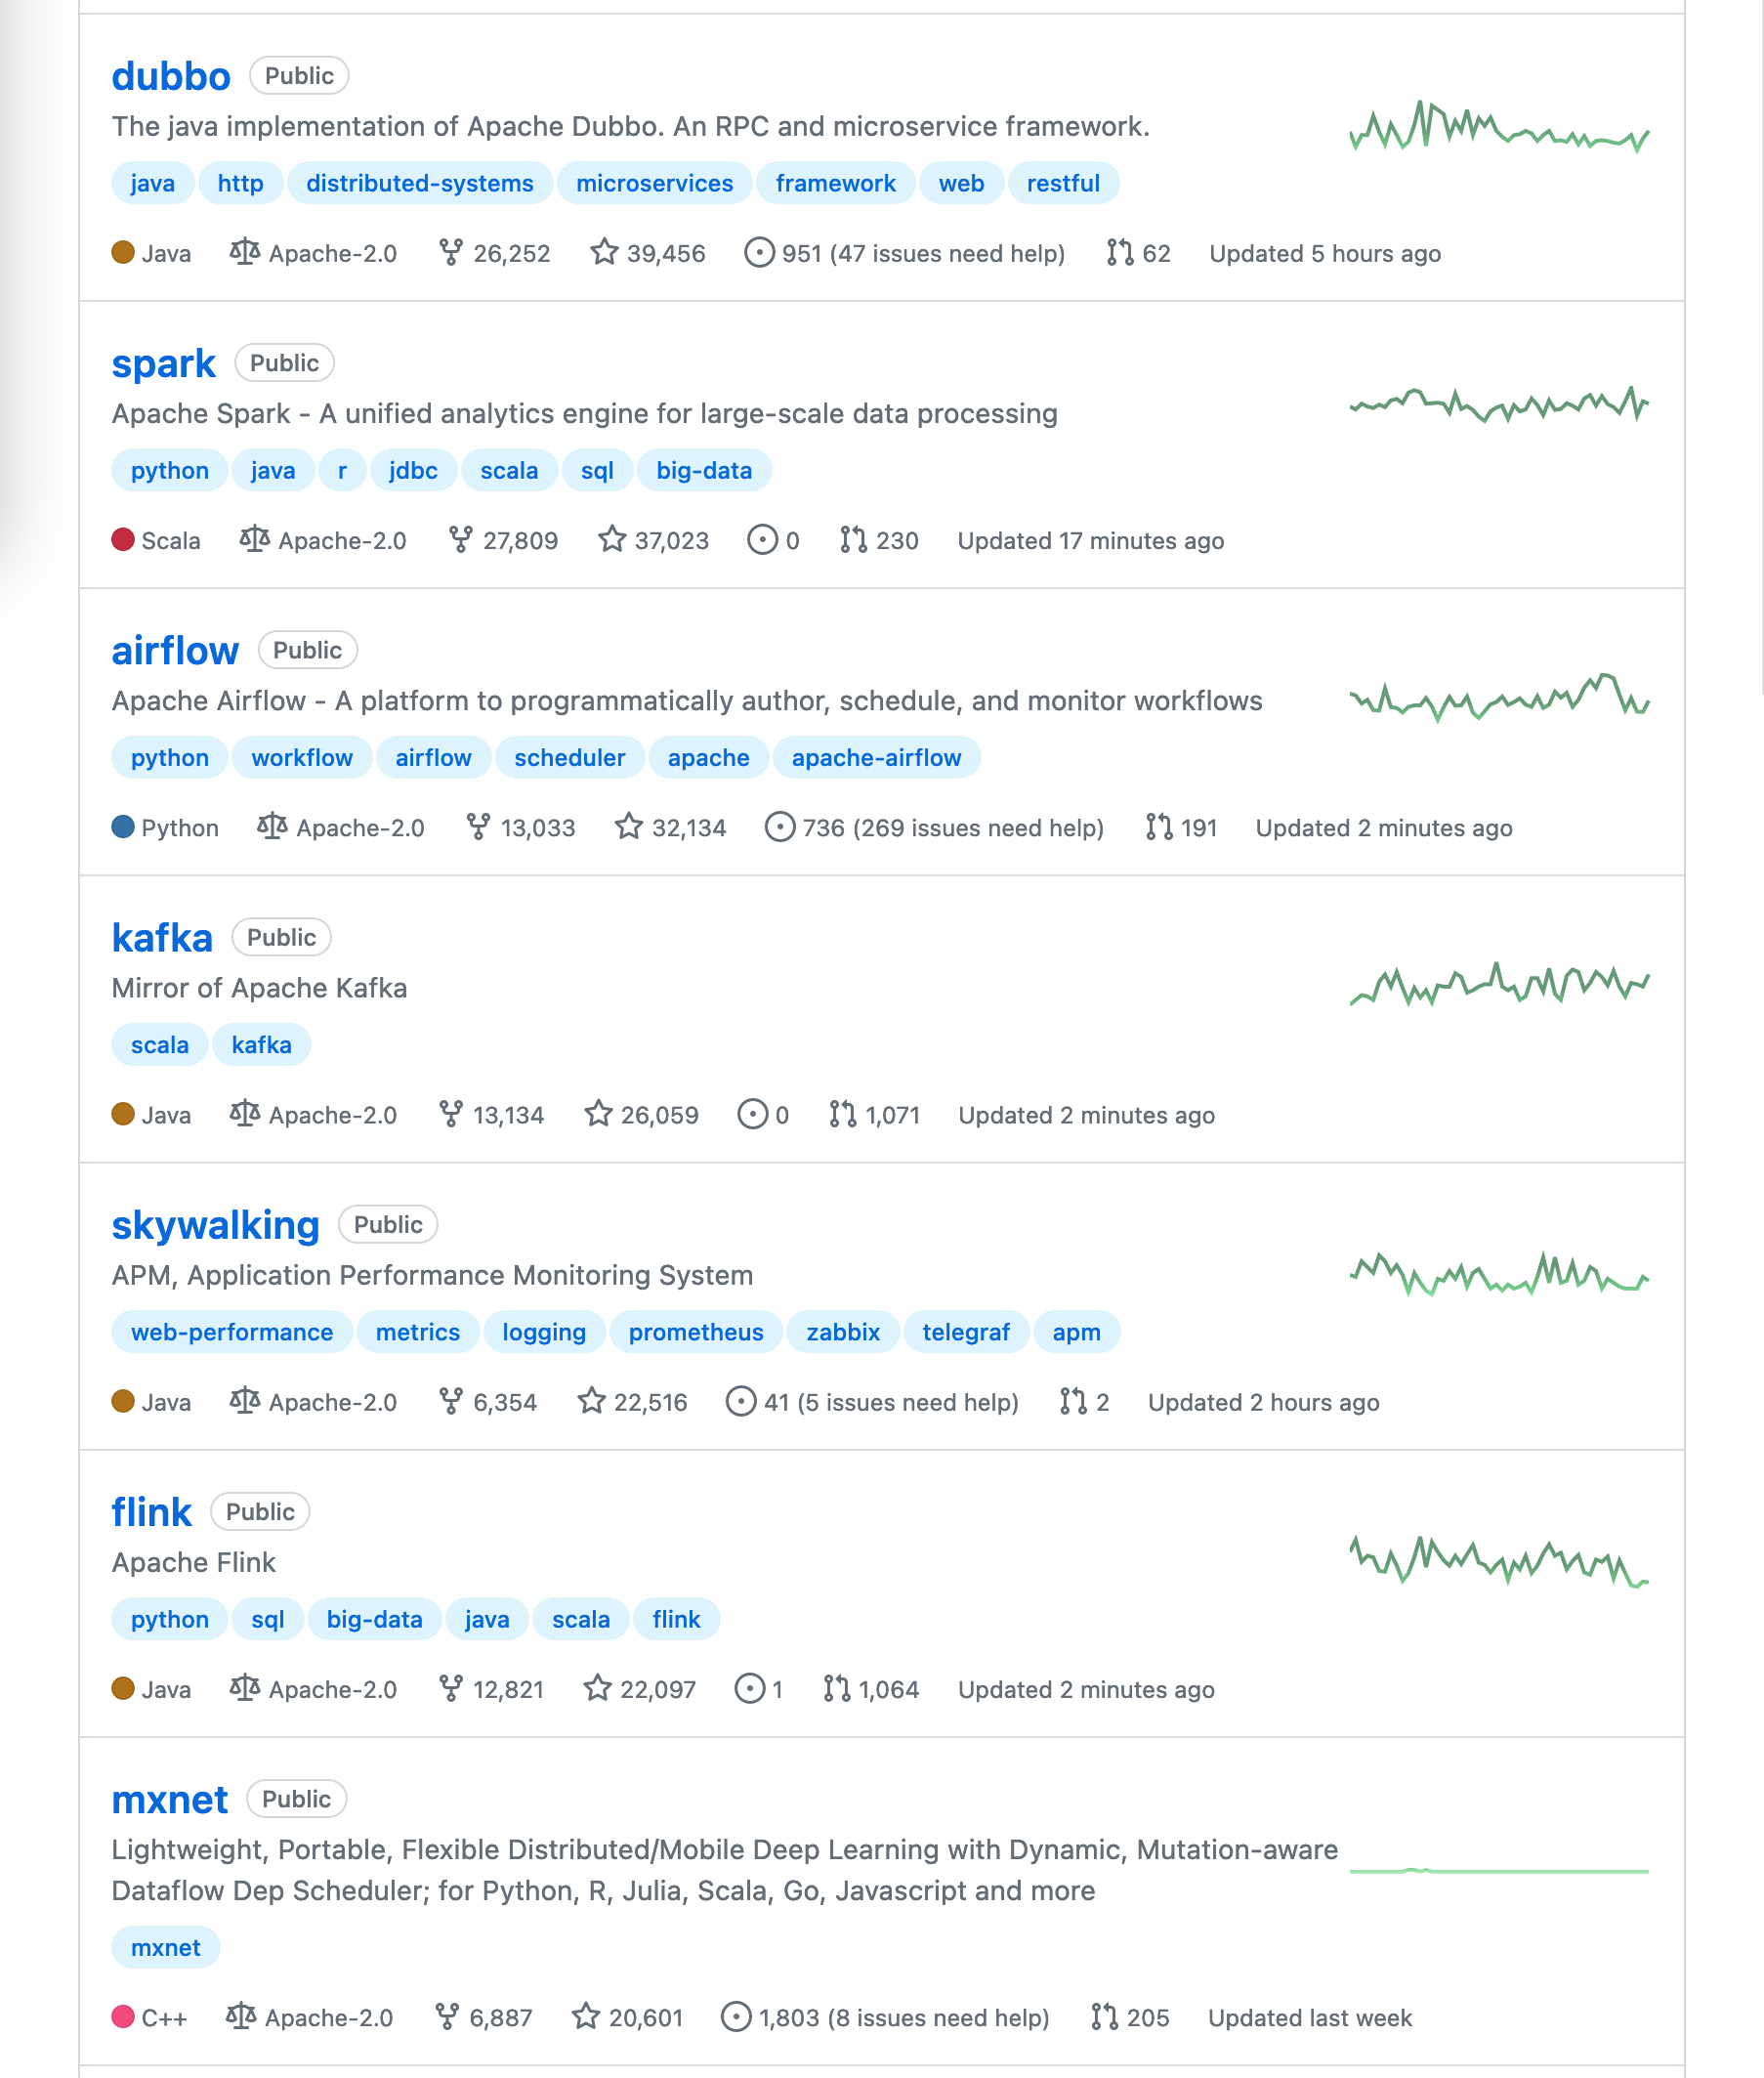
\includegraphics[width=40em]{beam-github-stars-dropdown-p2}
\end{center}
\WillContinue
\pagebreak

\Continuing
\begin{center}
    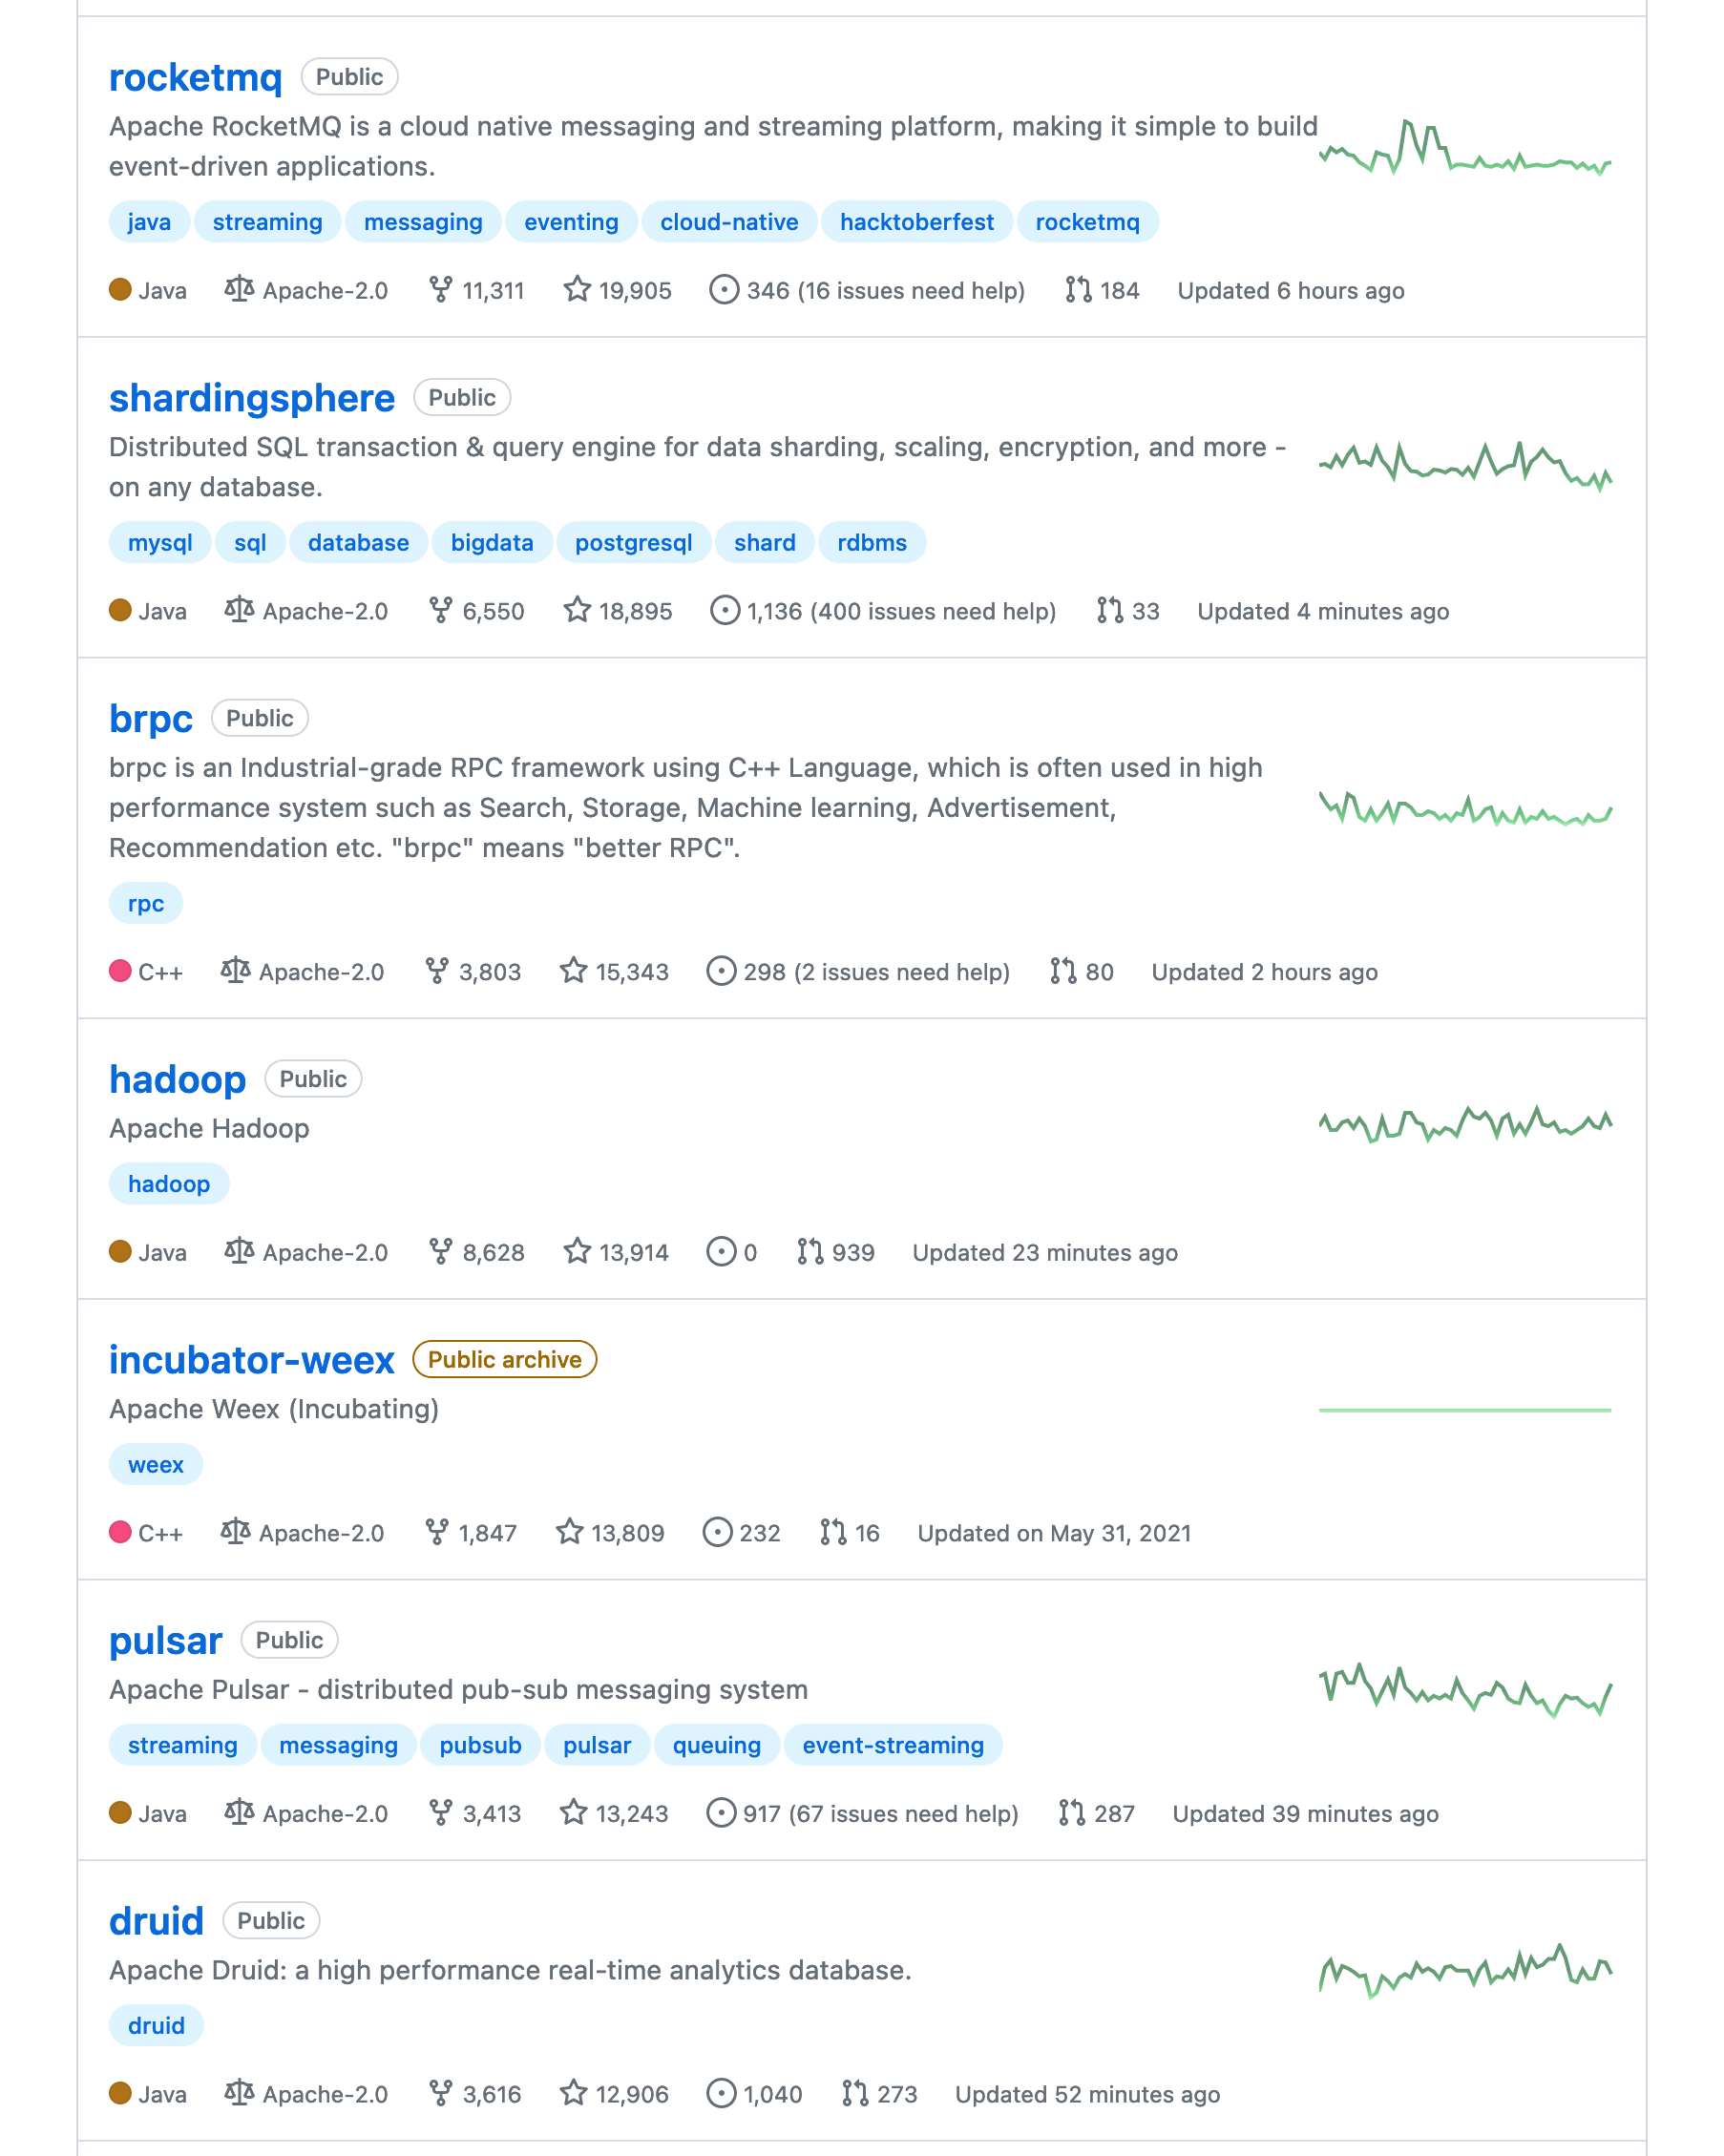
\includegraphics[width=40em]{beam-github-stars-dropdown-p3}
\end{center}
\WillContinue
\pagebreak

\Continuing
\begin{center}
    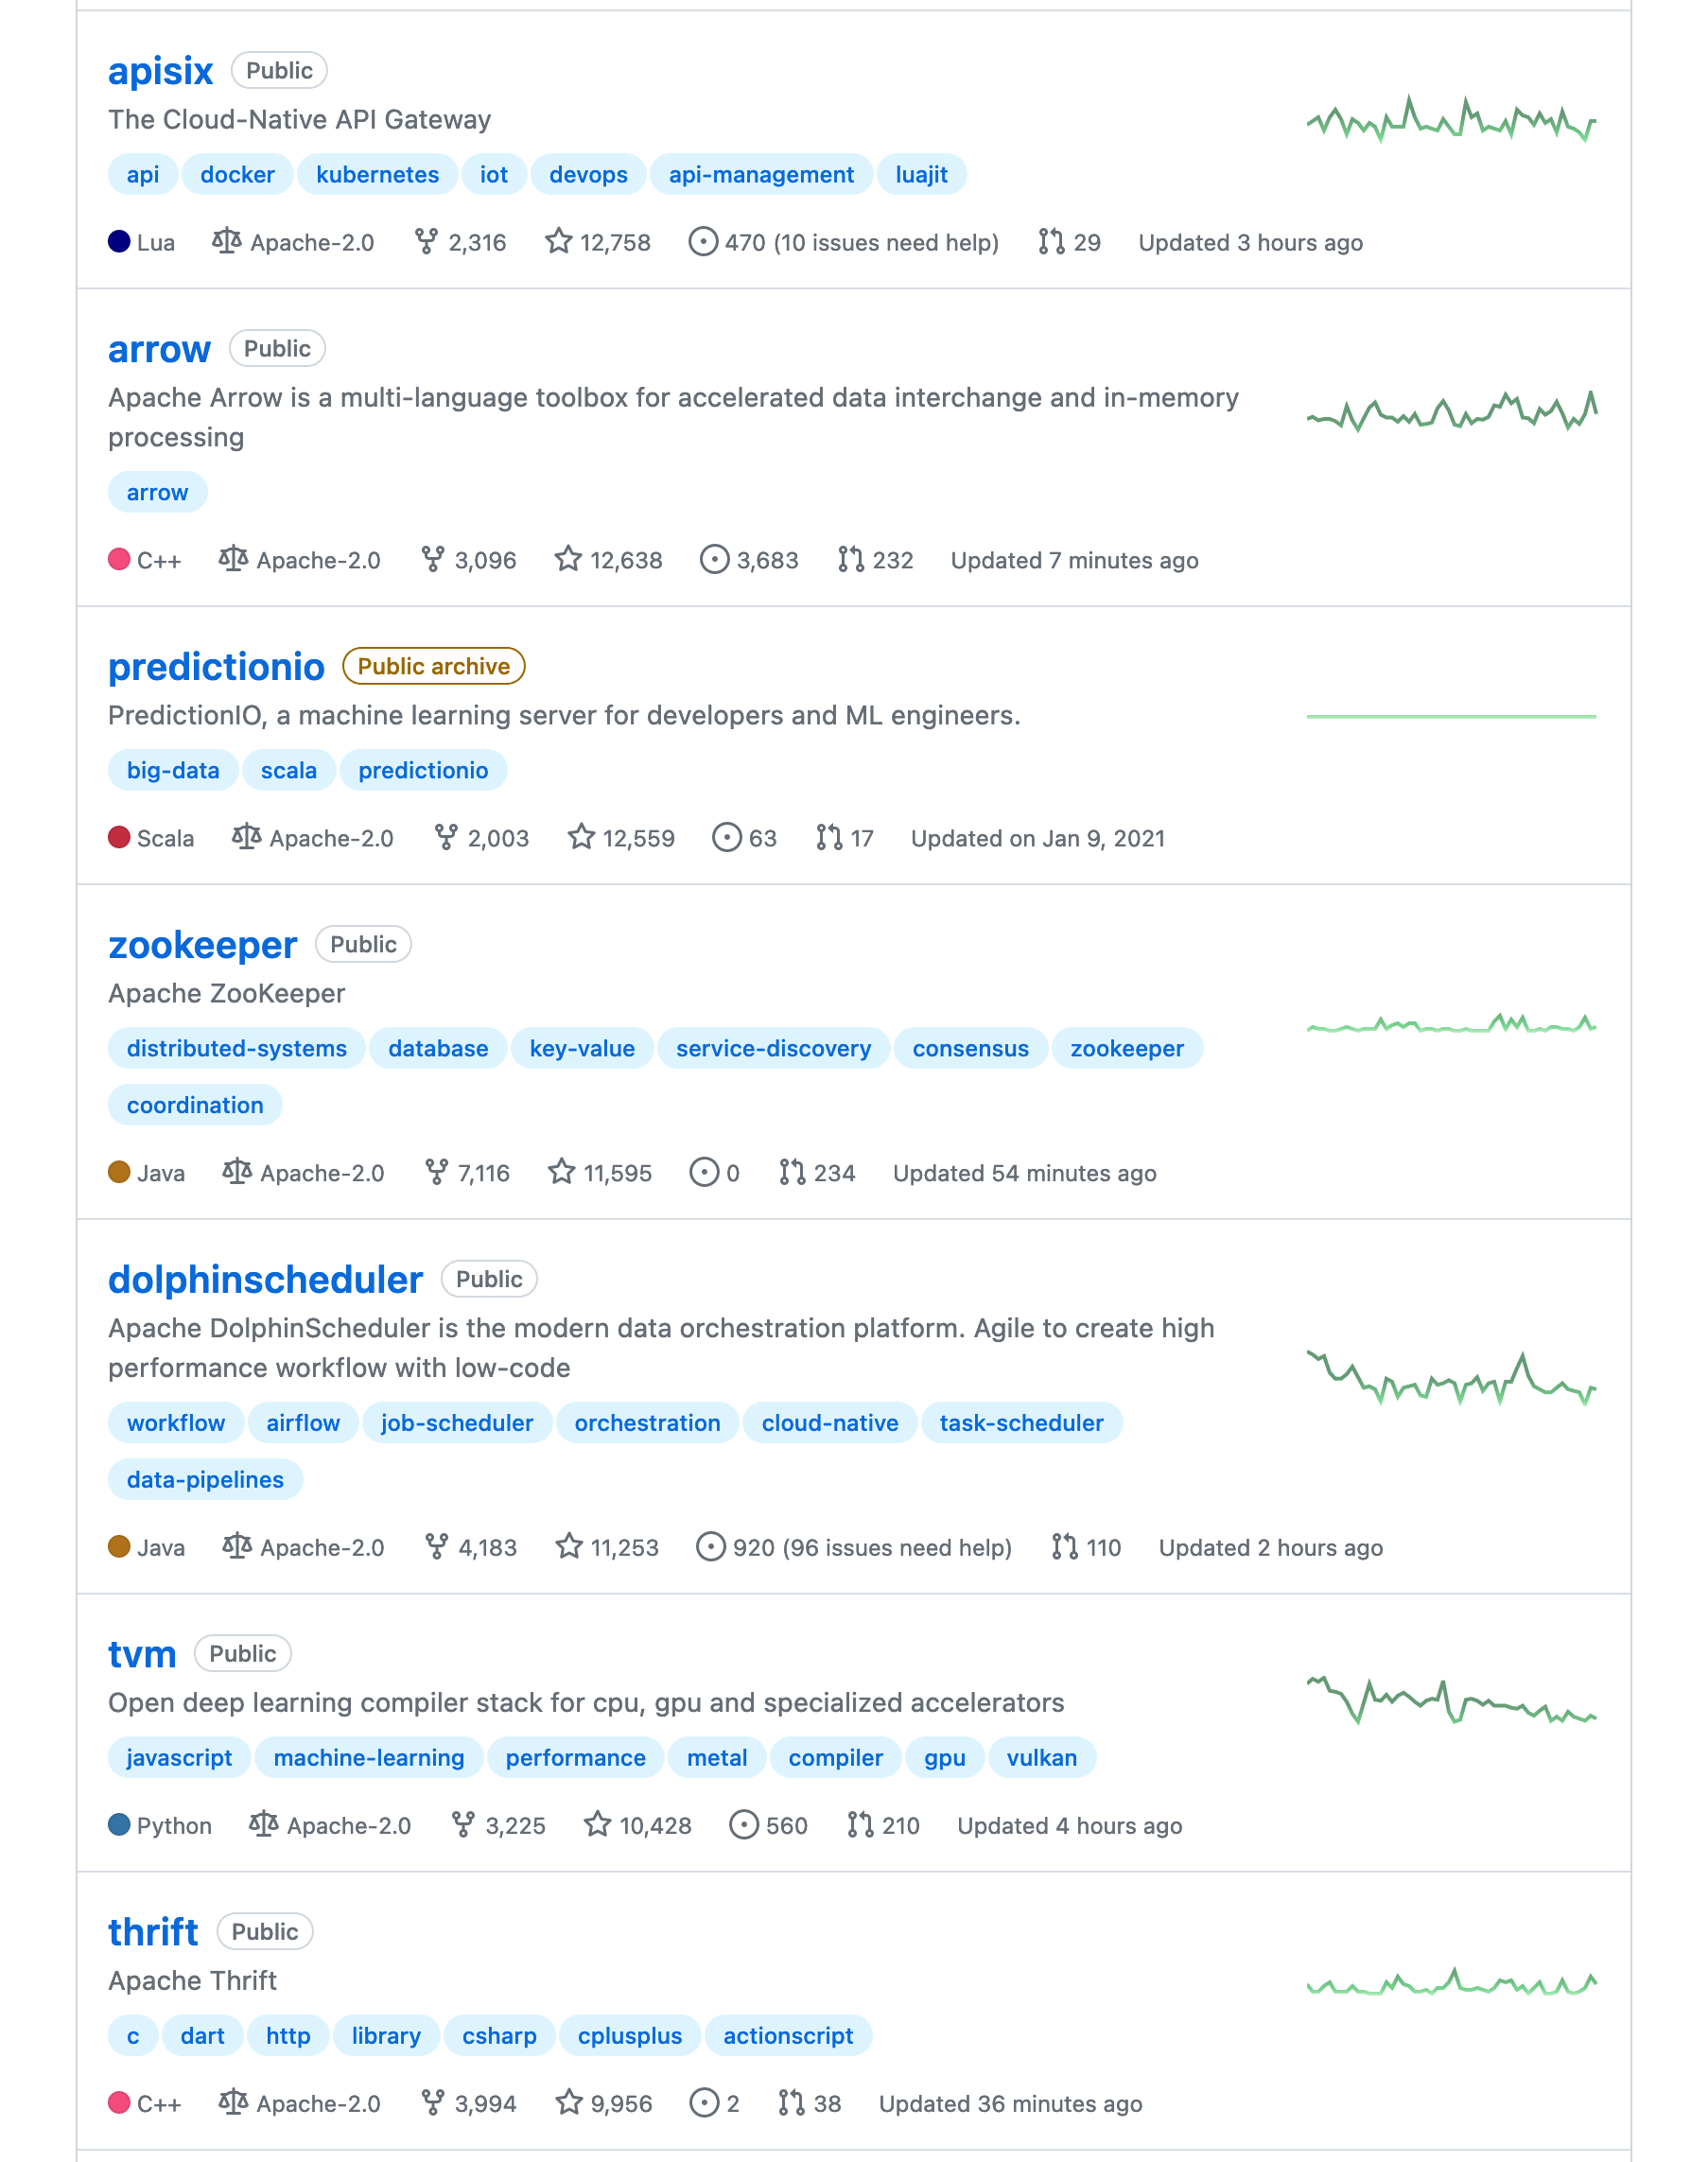
\includegraphics[width=40em]{beam-github-stars-dropdown-p4}
\end{center}
\WillContinue
\pagebreak

\Continuing
\begin{center}
    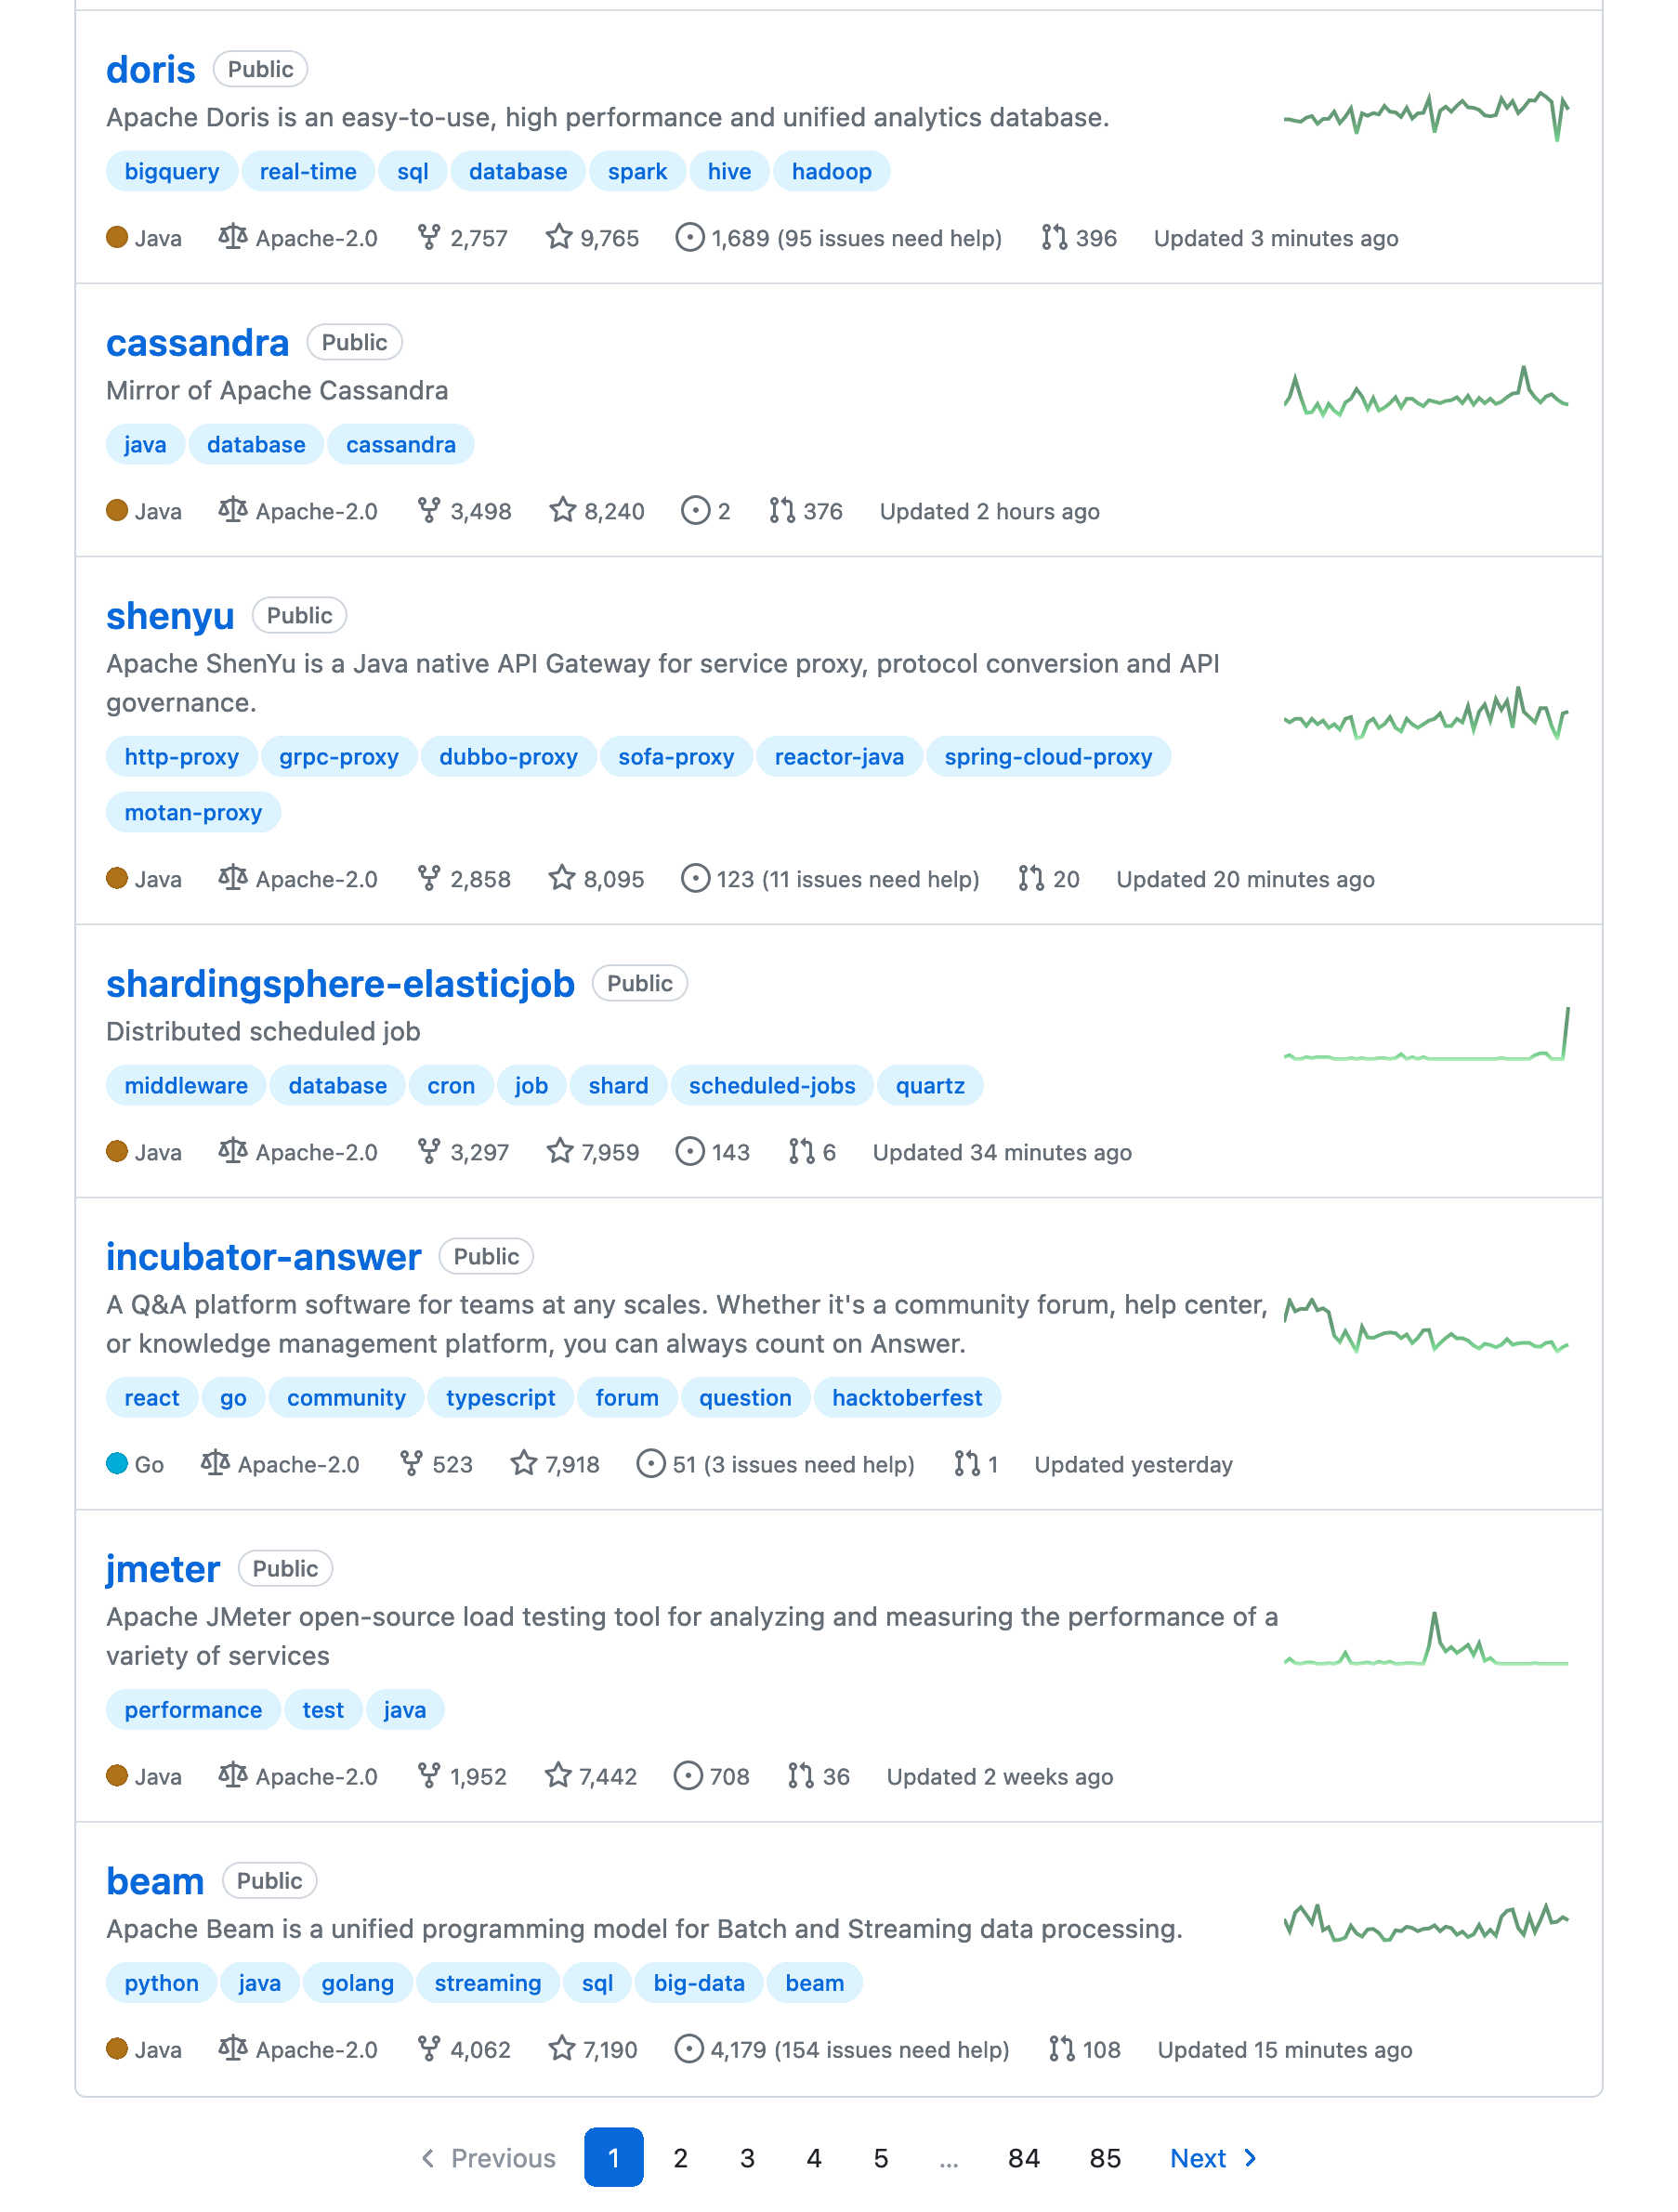
\includegraphics[width=40em]{beam-github-stars-dropdown-p5}
\end{center}

\pagebreak
